%LTeX: language=it
\subsection{UC 4 - Creazione contatto} \label{sec:UC4}
    \begin{itemize}
        \item \textbf{Attore principale}: MUA;
        \item \textbf{Descrizione}: il MUA deve poter creare un contatto nel sistema;
        \item \textbf{Precondizioni}: l’account che il MUA gestisce è registrato nel sistema, ha un connessione aperta con il sistema ed è autenticato;
        \item \textbf{Postcondizioni}: il MUA crea il contatto che viene salvato nel sistema;
        \item \textbf{Scenario principale}:
            \begin{enumerate}
                \item il MUA trasmette il nome del contatto (\hyperref[sec:UC4.1]{UC 4.1});
                \item il MUA trasmette l'indirizzo email del contatto (\hyperref[sec:UC4.2]{UC 4.2});
                \item il sistema salva il contatto;
            \end{enumerate}
        \item \textbf{Inclusioni}: nessuna;
        \item \textbf{Generalizzazioni}: nessuna;
        \item \textbf{Estensioni}:         
        \begin{enumerate}[label=\alph*.]
            \item il sistema non riesce a creare il contatto perchè il nome non è valido:
            \begin{enumerate}[label=\arabic*.]
                \item il sistema ritorna un errore al MUA di nome non valido (\hyperref[sec:UC4.3]{UC 4.3}).
            \end{enumerate}
            \item il sistema non riesce a creare il contatto perchè l'indirizzo email fornito non è valido:
            \begin{enumerate}[label=\arabic*.]
                \item il sistema ritorna un errore al MUA di indirizzo e-mail non valido (\hyperref[sec:UC4.4]{UC 4.4}).
            \end{enumerate}
        \end{enumerate}
    \end{itemize}

\begin{figure}[H]
    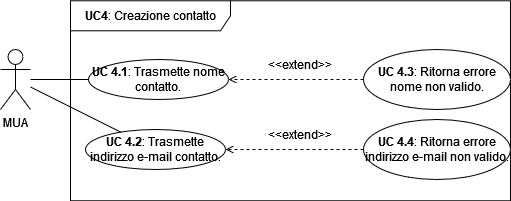
\includegraphics[width=0.85\textwidth]{sections/uc_imgs/UC04.png}
    \centering
    \caption{Diagramma sotto-casi UC 4}
\end{figure}

\subsubsection{UC 4.1 - Trasmette nome contatto} \label{sec:UC4.1}
    \begin{itemize}
        \item \textbf{Attore principale}: MUA;
        \item \textbf{Descrizione}: il MUA trasmette il nome per creare il contatto al sistema;
        \item \textbf{Precondizioni}: il MUA sta usando la funzionalità di creazione di un contatto;
        \item \textbf{Postcondizioni}: il sistema conosce il nome del contatto;
        \item \textbf{Scenario principale}:
            \begin{enumerate}
                \item il MUA invia il nome per creare il contatto al sistema;
                \item il sistema controlla che le informazioni ricevute rispettino il seguente requisito minimo:
                    \begin{itemize}
                        \item il nome del contatto non è una stringa vuota;
                    \end{itemize}
            \end{enumerate}
        \item \textbf{Inclusioni}: nessuna;
        \item \textbf{Generalizzazioni}: nessuna;
        \item \textbf{Estensioni}:
            \begin{enumerate}[label=\alph*.]
                \item il sistema non riesce a creare il contatto perché il nome fornito non è valido:
                \begin{enumerate}[label=\arabic*.]
                    \item il sistema ritorna un errore al MUA di nome non valido (\hyperref[sec:UC4.3]{UC 4.3}).
                \end{enumerate}
            \end{enumerate}
    \end{itemize}


    \subsubsection{UC 4.2 - Trasmette indirizzo e-mail contatto} \label{sec:UC4.2}
    \begin{itemize}
        \item \textbf{Attore principale}: MUA;
        \item \textbf{Descrizione}: il MUA trasmette l'indirizzo e-mail per creare il contatto al sistema;
        \item \textbf{Precondizioni}: il MUA sta usando la funzionalità di creazione di un contatto;
        \item \textbf{Postcondizioni}: il sistema conosce l'indirizzo e-mail del contatto;
        \item \textbf{Scenario principale}:
            \begin{enumerate}
                \item il MUA invia l'indirizzo e-mail per creare il contatto al sistema;
                \item il sistema controlla che le informazioni ricevute rispettino il seguente requisito minimo:
                    \begin{itemize}
                        \item l'indirizzo email del contatto non è una stringa vuota;
                    \end{itemize}
            \end{enumerate}
        \item \textbf{Inclusioni}: nessuna;
        \item \textbf{Generalizzazioni}: nessuna;
        \item \textbf{Estensioni}:
            \begin{enumerate}[label=\alph*.]
                \item il sistema non riesce a creare il contatto perché l'indirizzo e-mail fornito non è valido:
                \begin{enumerate}[label=\arabic*.]
                    \item il sistema ritorna un errore al MUA di indirizzo e-mail non valido (\hyperref[sec:UC4.4]{UC 4.4}).
                \end{enumerate}
            \end{enumerate}
    \end{itemize}




\subsubsection{UC 4.3 - Ritorna errore nome non valido} \label{sec:UC4.3}
    \begin{itemize}
        \item \textbf{Attore principale}: MUA;
        \item \textbf{Descrizione}: il sistema non riesce a salvare il contatto perché il nome del contatto non rispetta i requisiti;
        \item \textbf{Precondizioni}: il MUA ha inviato il nome del contatto;
        \item \textbf{Postcondizioni}: il sistema non salva il nuovo contatto, il MUA è stato notificato dell'errore;
        \item \textbf{Scenario principale}:
            \begin{enumerate}
                \item il sistema controlla la sintassi del nome del contatto e trova un errore;
                \item il sistema non salva il contatto e notifica il MUA dell'errore;
            \end{enumerate}
        \item \textbf{Inclusioni}: nessuna;
        \item \textbf{Generalizzazioni}: nessuna;
        \item \textbf{Estensioni}: nessuna.
    \end{itemize}

\subsubsection{UC 4.4 - Ritorna errore indirizzo e-mail non valido} \label{sec:UC4.4}
    \begin{itemize}
        \item \textbf{Attore principale}: MUA;
        \item \textbf{Descrizione}: il sistema non riesce a salvare il contatto perché l'indirizzo e-mail del contatto non rispetta i requisiti;
        \item \textbf{Precondizioni}: il MUA ha inviato l'indirizzo e-mail del contatto;
        \item \textbf{Postcondizioni}: il sistema non salva il nuovo contatto, il MUA è stato notificato dell'errore;
        \item \textbf{Scenario principale}:
            \begin{enumerate}
                \item il sistema controlla la sintassi dell'indirizzo e-mail del contatto e trova un errore;
                \item il sistema non salva il contatto e notifica il MUA dell'errore;
            \end{enumerate}
        \item \textbf{Inclusioni}: nessuna;
        \item \textbf{Generalizzazioni}: nessuna;
        \item \textbf{Estensioni}: nessuna.
    \end{itemize}